% 页数安排:10 10 15 20 20 3 + 15(prefix) + 10(suffix) = 103
% 基于Web-Service的开放式陆地生态系统碳循环模型对比系统构建方法研究
% 开放式陆地生态系统碳循环模型对比系统构建方法研究
\chapter{绪论}
\section{研究背景及意义}
\subsection{研究背景}
% - 介绍全球变化、气候变暖现象,为解决该现象出现的地球系统模式(气候系统模式),陆地生态系统碳循环模型在其中扮演的角色
% - 介绍陆地生态系统碳循环模型的概念、发展、研究现状、对比
% - (碳)模型对比——热点和难点
% - 介绍新兴技术及对碳循环模型对比的意义
% - 总结开放式对比的热点、难点、意义

自工业革命以来,人类活动正在大规模地改变陆地生物圈结构,其中最典型的是温室气体浓度尤其是$CO_2$浓度增加导致的全球气候变暖~\cite{houghton2001climate}。据预测,如果温室气体以目前的排放速率持续下去,地表温度将可能每10年上升0.2℃,100年后的全球平均温度将大约增加2℃(变异范围为1.4\textasciitilde5.8℃)~\cite{Oliver2013Intergovernmental}~\cite{宋燕燕2006陆地碳循环模型的比较分析},由此将会进一步引发一系列严重的全球问题,对人类的发展和社会经济的持续发展带来巨大的威胁。

为了合理预测气候变化特别是全球变暖对生态系统造成的影响,必须深入研究地球系统碳循环过程。而碳循环模型是模拟生态系统,估计和预测不同尺度碳收支格局和变化的重要手段~\cite{cao2003interannual}。从碳循环的完整流程上来看,地球(气候)系统模式包括了碳在海洋、大气、化石、陆地等生态系统中的完整循环流程,是模拟碳循环过程的有效工具。而其中陆地生态系统作为人类活动的聚集地,是四大碳库中最为活跃的一个碳库。陆地生态系统碳循环模型通过对光合作用、呼吸作用、土壤呼吸等过程的对碳循环进行模拟,对植被生产力的模拟和耦合气候模式评估气候变化具有重要作用。

% 以陆地生态系统碳循环领域为例,为了模拟生态系统中大气、海洋、陆表和化石燃料四个碳库之间的碳循环过程,预测不同尺度的碳收支格局和变化情况(Cao M K et al., 2005;Cao,et al.,2003),大气学家研发了众多的碳循环模型,大致可以分为统计模型、遥感参数模型、生态过程模型和遥感、过程耦合模型四类。代表性的有Miami模型~\cite{Lieth1975Primary}、CASA~\cite{Potter1999Interannual}~\cite{Potter2003Continental}、GLO-PEM~\cite{Prince1995Global}~\cite{Goetz2000Interannual}、BIOME-BGC~\cite{running1988general}~\cite{Running1991FOREST}~\cite{thornton2000user}、IBIS(Foley et al., 1996)、LPJ DGVM~\cite{Gerten2004Terrestrial}~\cite{Sitch2010Evaluation}等。各个模型由于其模拟机理不同,有其各自适用的尺度和范围。

陆地生态系统碳循环模型从上世纪90年代以统计模型为代表的兴起,到如今已经经历了长足的发展,从类别上可大致分为统计模型、遥感参数模型、生态过程模型和遥感过程耦合模型。然而,由于碳循环模型涉及到的生物、物理、化学和地球机理的复杂性,各个模型有其各自的适用时空尺度的先决条件,在应用时往往难以进行选择,其模拟结果也不尽相同。为了评估气候模型的适用情景、模拟效果、参数敏感性和气候的历史规律及未来趋势,世界气候研究计划(WCAR,World Climate Research Programme)组织了6次耦合模型对比计划(CMIP,Coupled Model Intercomparison Project),针对每届IPCC(IPCC,Intergovernmental Panel on Climate Change)评估报告中出现的科学问题制定标准实验方案,对比各个模型的模拟能力~\cite{meehl2000coupled}。其中,目前正在开展的第六阶段耦合模型对比计划(CMIP6)背书的模型对比项目有23余个,包括气溶胶和化学模型对比项目、耦合气候碳循环模型对比项目、云反馈模型对比项目、十年际气候预测项目、海洋模型对比项目、古气候模型对比项目、辐射强迫模型对比项目等~\cite{eyring2016overview}~\cite{WCRP-CMIP6-Endorsed-CMIPs}。除此此外,区域气候模型评估系统(RCMES,Regional Climate Model Evaluation System)和协调区域气候降尺度实验(CORDEX,Coordinated Reginal Climate Downscaling Experiment)也在区域尺度上开展气候模型的对比评估,通过区域尺度上的评估决策弥合全球尺度上的气候变化~\cite{loikith2013scientific}。在陆地碳循环领域,全球分析、集成和建模(GAIM, Global Analysis, Integration, and Modelling)工作组和生态系统模型数据对比计划对植被净第一性生产力(NPP,Net Primary Productivity)进行了对比。
可见,模型对比评价是当前碳循环研究领域的一个\textbf{热点}。但是,现有的对比计划大多数都是针对气候系统模式模拟的地球系统碳循环,针对陆地生态系统碳循环模型的对比还相对较少。

据统计,在第五次耦合模型比较计划(CMIP5)中,超过20个建模组使用50多个碳循环模型参与模拟~\cite{Taylor2012An};在GAIM对比项目中,超过15个陆地碳循环模型参与对比~\cite{cramer1999comparing}~\cite{kicklighter1999comparing},
越来越多的模型参与到对比计划中。但是,模型对比仍然面临着诸多困难:

\begin{enumerate}[(1)]
    \item \textbf{从碳循环的过程上来看},碳循环模型通常涉及到生物(光合作用、呼吸作用)、物理(植被冠层能量交换)、化学(碳、水循环)、遥感(数据同化)等模块,每个模型由于其机理不同,涉及到的模块组成往往不同,而且各个模块的实现方法也不尽相同;
    \item \textbf{从模型开发视角上来看},碳循环模型由不同的科研人员编写,面临着操作系统、编程语言、软硬件环境依赖、运行方式、输入输出数据格式等多方面的异构性,难以部署、编译和应用,阻碍了模型的推广;
    \item \textbf{从数据搜集上来看},不同的碳循环模型需要的驱动数据不尽相同,在模型对比时需要在数据搜集和预处理上耗费巨大的精力;
    \item \textbf{从模型对比的层面上来看},碳循环模型的对比应该从多个层面上开展,包括单个观测站点层面、不同植被功能类型的差异性和全球范围的时空分布格局等。
\end{enumerate}

这些原因共同限制了模型对比工作的发展,模型对比也是当前碳循环模型研究领域的一个\textbf{难点}。

随着计算机和网络技术的发展,Web Service和面向服务的软件架构(SOA,Service-Oriented Architecture)技术不断成熟,地理模型和数据逐渐朝着网络服务化的方向进行封装与共享~\cite{adgeo-4-69-2005}~\cite{peckham2009componentizing}~\cite{胡迪2015地理模型的服务化封装方法研究},为碳循环模型对比过程中面临的难点提供了技术上的有效支撑。服务化的地理模型将复杂的地理模型封装为一个黑箱,屏蔽了模型在机理上和操作上的复杂性和异构性,大大降低了碳循环模型的应用难度~\cite{胡迪2015地理模型的服务化封装方法研究}~\cite{yue2016service};地理数据服务不仅可以降低数据搜集的困难,更重要的是解决了网络环境下数据与模型难以互操作的问题~\cite{Yue2015A}。
\textbf{本文基于微服务的分布式网络架构,设计了一套高效稳定可用的陆地生态系统碳循环模型对比框架,开放了一系列模型资源、数据资源和对比资源服务化接入接口,通过科学工作流驱动模型服务、数据服务和对比服务的集成互操作,实现了陆地生态系统碳循环模型的对比。}

\subsection{研究意义}
% - 通用的意义:开放、公平、可共享、可重用。
% - 对碳循环模型的意义:促进碳循环模型的发展改进,提高碳循环模型的精度,提高人们对碳排放的认知,为解决气候问题提供准确有效的模拟手段。

本文基于网络服务开展模型的对比,通过模型资源、数据资源和对比方法及方案的服务化封装、部署、发布、共享和集成,为陆地生态系统碳循环的对比提供了一种新的方案。对于陆地生态系统碳循环模型来说,屏蔽了彼此之间的异构性和复杂性,实现了模型资源的共享,促进了模型的应用推广和发展;对比碳循环相关数据来说,降低了数据收集、存储、管理、处理的繁琐流程;对于模型对比来说,一方面可以将传统的线下对比过程公开化、透明化,使对比过程具有可追溯性、可验证性和易重复性,另一方面对比方案也可以共享出来,在研究不同时空尺度的地区时,可以重用起来。

\section{国内外研究现状综述}
陆地生态系统碳循环模型对比的一系列难点在很大程度上来源于模型的复杂性和异构性,而模型服务的封装发布屏蔽了这一点。因此,本文从现有的陆地生态系统碳循环模型的起源、发展、应用、对比入手,回顾前人在模型对比、地理模型服务、地理数据服务和服务集成应用等方面所做的工作,分析陆地生态系统碳循环领域地理模型对比的研究现状、存在问题和发展趋势。

\subsection{陆地生态系统碳循环模型及其对比}
% 模型起源-发展-应用-扯到对比-单模型的对比-多模型的对比
% 模型对比模式,几个例子
自从20世纪50年代Craig~\cite{craig1957natural}在全球碳循环模式中使用两个碳库模拟陆地生态系统的碳平衡以来,经过Emanuel等~\cite{emanuel1985climatic}对陆地生态系统在全球碳循环中的作用模式的早期探索,陆地生态系统碳循环模型的研究取得了极大的发展。陆地碳循环模型可以简单分为统计模型、生态过程模型和遥感过程耦合模型。统计模型可分为气候统计模型和遥感统计模型。其中气候统计模型主要通过在气候因子与植被净初级生产力(Net Primary Productivity,NPP)的实测数据之间建立回归方程;遥感统计模型通过遥感光谱指数(如NDVI)与NPP、生物量等数据间的相关关系进行统计回归。统计模型简单直观,具有较强的区域适用性,但其完全依赖于地面观测数据,对于不同的区域,模型不具备普适性和推广性。同时统计模型没有考虑陆地生态系统碳循环过程的内部机理,无法揭示生态系统与环境间的相互影响关系,不能用于对未来的预测研究~\cite{袁文平2014陆地生态系统植被生产力遥感模型研究进展}~\cite{谢馨瑶2018大尺度森林碳循环过程模拟模型综述}。生态过程模型按照是否考虑实际环境对植被类型、组成和结构的影响分为基于动态植被类型的模型和基于静态植被类型的模型~\cite{王绍刚2008森林碳循环模型方法研究进展}~\cite{王萍2009森林碳循环模型概述}~\cite{毛留喜2006陆地生态系统碳循环模型研究概述},按照涉及到的机理类型分为地球化学过程模型、陆面物理过程模型和生物过程模型~\cite{谢馨瑶2018大尺度森林碳循环过程模拟模型综述}。过程模型由于其综合考虑了碳循环过程的动力学特征,结合了气候、土壤和植被生理生态参数,以及陆地生态系统与大气、海洋之间的相互作用,模拟结果相对来说更加准确,逐渐占据了主导地位。遥感、过程耦合模型通过将遥感观测数据(如叶面积指数LAI)同化到模型之中,来提高模型模拟的精度~\cite{2013基于数据同化的哈佛森林地区水、碳通量模拟},他融合了遥感统计模型和生态过程模型的优点,可以反映区域和全球尺度的NPP空间分布和变化~\cite{朱文泉2005陆地植被净初级生产力计算模型研究进展}。
对于陆地生态系统碳循环模型的对比,可以简单分为两类:一是单个模型在开发和应用时与涡度通量观测点、文献记录和遥感数据的对比;二是在多个模型之间开展对比计划。

对于单个模型的对比验证,Kucharik等~\cite{Kucharik2000Testing}将IBIS模拟NPP、生物质、叶面积指数等指标,与12种植被类型的通量观测数据向对比,发现NPP在温带落叶林的误差最小,为4.0\%,而在北方混交林的误差最大,为89\%,平均误差为39\%,总体来说IBIS适用于区域尺度和全球尺度的生态模拟。杨延征~\cite{杨延征2016基于}、刘曦~\cite{刘曦2011IBIS}、王磊~\cite{2010基于}、张海燕~\cite{2009应用}等人使用IBIS分别在中国全国范围、中国东北东部森林、中国东部和东北帽儿山应用IBIS模型估算碳排放情况,分别将模型模拟的结果与已发表的文献、通量站点观测数据对比,结果表明IBIS模拟的NPP结果都在合理的误差范围内,验证了其在中国各种植被类型下都具有很好的模拟能力。
% 张延龙、郑磊、胡波等使用Biome-BGC分别在哈佛森林、阔叶红松林生态系统、黄淮海地区模拟NPP,
Kimball~\cite{kimball1997biome}使用Biome-BGC模拟北方林地的水通量,结果表明模拟的径流量和土壤水通量决定系数在62 \textasciitilde 98\%之间;Venevsky~\cite{venevsky2007sever}对LPJ模型进行了改进,将时间步长由1月改为了1天,并与欧洲通量网的13个站点观测的NEE进行对比,模拟的决定系数$R^2$为0.59,具有很好的准确度。

% 胡瀞予(2011)、NIU Ben~\cite{Niu2017Satellite}等人分别以台湾陆域生态区和青藏高原为研究区域,将生物测定法、Rahman’s方程式以及VPM、PCM、AVM的模拟结果与MOD17数据集相对比,评估其模拟能力。

对于多个模型之间的对比计划,在全球碳循环模型方面,世界气候研究计划开展的CMIP~\cite{meehl2000coupled}~\cite{Taylor2012An}~\cite{eyring2016overview}最为完善,它设计了一系列诊断试验,这些试验包括一些必做项目,比如历史模拟和4个DECK(Diagnostic,Evaluation and Characterization of Klima experiments)试验,参与对比的模式组模拟这些试验,并将结果提交给评委组,通过评审后将对比结果公布出来~\cite{赵宗慈2016CMIP6}。为确保模型最大化地使用相同的驱动数据,CMIP通过地球系统网格联盟(Earth System Grid Federation,ESGF)~\cite{williams2011earth}向模式组提供通用的输入数据(input4MIPs)和观测数据(obs4MIPs)来支持模型的运行和对比;对于陆地碳循环的对比,Cramer等人~\cite{cramer1999comparing}~\cite{kicklighter1999comparing}~\cite{bondeau1999comparing}开展的GAIM项目综合对比了三类共15个陆地生态系统碳循环模型:a). 基于遥感数据的光能利用率模型(CASA,GLO-PEM,SDBM,SIB2和TURC);b). 静态植被类型模型(Biome-BGC,CARAIB 2.1,CENTURY 4.0,FBM 2.2,HRBM 3.0,KGBM,PLAI 0.2,SILVAN 2.2和TEM 4.0);c). 动态植被类型模型(BIOME3,DOLY和HYBRID 3.0)。GAIM的对比通过使用相同的驱动数据集,使用统一的可视化工具来保证对比的公平性。

% 对于陆地生态系统碳循环模型模拟结果的验证和对比,前人大多从多个视角进行综合对比,包括对模拟结果的可视化观察对比,使用统计学方法定量地对比等。没有单独的评价手段被认为是优越的,相反的,多种对比技术的结合使用能够为模型模拟能力提供全面评价~\cite{Taylor2012An}。

%在对比对象方面,目前主要分为三类:基于通量站点数据的对比、基于卫星遥感数据的对比和基于多模型模拟结果的交叉对比。P.Friedlingstein(2006)在CMIP4中通过11个碳循环模型之间模拟结果的相互比较来评价其模拟能力。

%在对比方法方面,通过绘制模拟值等值线图、观测值等值线图、差异等值线图可以非常直观地展示出各个模型模拟结果的差异;通过泰勒图展示模拟值与观测值之间的标准差之比、均方根误差以及相关系数;通过纵向图和时间序列折线图可以清晰地展现模型在各个子区域中的适用情况~\cite{Kim2013Evaluation}~\cite{Kim2014Evaluation}~\cite{Kim2017Winter}~\cite{刘敏200913}(Kim J,2012;Kim J,2014;Kim J,2018;郭彦,2013;刘敏,2009)。Stoner A M K~\cite{Stoner2013An}使用统计降尺度的方法建立当前观察值、当前模拟值、未来模拟值与未来观察值之间的关系,预测未来的气候因子发展状态。

% 在对比框架方面,国际上比较知名的是WCAR开展的CMIP。通过制定一系列证明模型模拟能力的标准实验,参与比较的模型都遵循实验协议进行测试。使用一致的预测因子(如数据源、空间分辨率、时间分辨率等),针对特定的预测指标(如温度、湿度、降水量、NPP等),在一致的时间范围内模拟,最后将模拟结果提交给专家评审,通过审核的对比结果被公开发布在网站上~\cite{Taylor2012An}。耦合模型对比计划、协调区域降尺度实验以及区域气候模型评估系统都遵循着这种对比框架开展对比~\cite{eyring2016overview}~\cite{Gutowski2009The}~\cite{赵宗慈2016CMIP6}。

\subsection{地理数据服务和地理模型服务}
随着计算机网络的高速发展,人们希望能够通过互联网获取与自己息息相关的地理空间数据,但由于地理数据的非结构化异构特征,难以进行解析、查询和可视化。开放地理空间信息联盟(OGC)开展了OpenGIS网络服务(OWS)研究计划,其目的是通过提供一个与具体厂商无关的互操作框架,实现各种地理数据和地理处理功能在互联网上的发现、存取、利用和可视化等~\cite{lake2009infrastructure}。目前,在地理数据服务和地理模型服务的理论、方法和标准规范方面均取得了可喜的成果。在地理数据服务方面,以WMS(Web Map Service)、WFS(Web Feature Service)、WCS(Web Coverage Service)为代表分别实现了网络地图的显示、矢量数据、栅格数据的空间互操作~\cite{OGC-WMS}~\cite{OGC-WCS}~\cite{OGC-WFS}。在地理数据表达标准方面也有一些规范,包括矢量数据的表达规范有GML(Geography Markup Language)、KML(Keyhole Markup Language)、GeoJSON、TopoJSON、SVG(Scalable Vector Graphics)等~\cite{GML}~\cite{KML},地理坐标和投影的表达规范WKT(Well-Known Text)等~\cite{lott2015geographic}。针对地理模型与地理数据在集成时难以适配和耦合的问题,乐松山~\cite{Yue2015A}~\cite{Yue2013Key}~\cite{yue2015data}~\cite{wang2018study}~\cite{乐松山2016面向地理模型共享与集成的数据适配方法研究}提出了通用数据表达——交换模型(UDX)表达地理数据,并以一系列与之配套的数据映射服务、数据重构服务进行数据适配,以语义概念资源库、空间参考资源库、单位量纲资源库和通用数据表达模板库对数据进行语义内涵描述。

与地理数据服务相比,地理模型服务的起步较晚,应用面也稍窄一些。OGC针对网络环境下的地理处理需求设计了WPS(Web Processing Service)规范,致力于实现GIS功能的服务化调用~\cite{OGC-WPS}。胡迪~\cite{胡迪2015地理模型的服务化封装方法研究}通过输入输出重定向、操作系统文件拦截和图形用户界面自动化测试3中方法实现了具有复杂交互方式的地理模型的服务化封装。吴楠~\cite{吴楠2012基于}、毛曦~\cite{毛曦2012基于}、宋东泽~\cite{宋东泽2015一个生态传感网的}等基于WPS标准,分别实现了VPM模型和日均蒸散量模型的服务发布。

\subsection{模型和数据服务集成应用}
由于地理现象的复杂性,在实际地理建模和模拟时往往需要多个模型集成耦合,地理服务集成应用框架逐渐发展起来。OpenMI(Open Modelling Interface)~\cite{MOORE2005279}~\cite{gregersen2007openmi}通过对数据标准的定义、描述和传递,实现了复杂水文模型的集成,目前OpenMI已经被OGC认可并推广为地理模型集成标准。乐松山等~\cite{yue2016service}~\cite{zhang2019design}~\cite{wen2017model}~\cite{yue2018loosely}设计了一套模型服务封装、发布和集成的标准,实现了分布式网络环境下多源异构地理模型和数据的集成应用。CSDMS(Community Surface Dynamics Modeling System)~\cite{Peckham2013A}~\cite{peckham2009componentizing}采用组件化的方式对地表过程模型进行集成耦合,并以网络服务提供操作接口。


\subsection{研究现状分析与总结}
\begin{enumerate}[(1)]
\item \textbf{陆地生态系统碳循环模型及其对比:}

纵观陆地生态系统碳循环模型起源、发展和应用,越来越多的陆地生态系统碳循环模型被开发出来。面对种类繁多的碳循环模型,国内学者在多模型对比方面所关注较少,更多是进行单模型的验证对比上;国外学者在全球碳循环的对比方面开展过多次研究,但在陆地碳循环方面相对较少。在对比方案上,一致认同的是尽可能地都采用相同的驱动数据模拟,对于非公共输入数据项,要求将其一并提交给评审委员会,并公开发布出去。对比试验由各个模式组分别完成,最后提交给评委。
这种对比方案已经趋向成熟,但是对比过程完全由评审委员会和模式组参与,相对来说不够公开透明;对比范围广阔但同时周期又过长,CMIP6的完成预计需要5年时间直到2020年才结束;当出现新的研究区域时对比过程难以重现。这种对比方案有进一步完善的空间。  % TODO

\item \textbf{地理数据服务和地理模型服务:}

在互联网技术浪潮的推动下,地理数据和地理模型在网络服务方向也高速发展。在以OGC为代表的各种研究机构的推动下,当前在数据标准描述方法和数据服务方面已经逐渐完整和完善,在模型服务的发布方面技术也已成熟,越来越多的地理模型在网络环境下应用起来。但是,陆地生态系统碳循环模型服务和数据服务的应用还相对较少。

\item \textbf{地理服务集成应用框架:}
% OGS WPS 标准的缺点:
% 数据基于栅格和GML
% 不支持模型集成

在地理服务的集成应用方面,目前也有了多种解决方案。但是,服务集成应用框架往往受限于服务封装标准和领域应用标准,在陆地生态系统碳循环的集成应用和服务化对比方面还缺乏研究。

\end{enumerate}

\section{研究目标与研究内容}
\subsection{研究目标}
针对当前陆地生态系统碳循环模型在对比时面临的主要难点,即模型和数据的异构性,提出通过地理模型和数据的封装、发布、共享、集成来实现模型对比。具体研究目标包括:
% 这里和下文研究内容不太对应
\begin{enumerate}[(1)]
    \item 设计一套基于网络服务的高效稳定可用的陆地生态系统碳循环模型对比系统框架,支持各种模型和数据的开放式接入;
    \item 设计陆地生态系统碳循环相关数据、模型及对比资源的结构化描述方法和服务化方法;
    \item 以IBIS、Biome-BGC和LPJ三个陆地生态系统碳循环模型为例,从观测站点、植被功能类型和全球时空分布格局三层上进行对比,分析三个模型的模拟效果,验证系统的可用性。
\end{enumerate}

\subsection{研究内容}
为实现上述研究目标,设计研究内容如下:
\begin{enumerate}[(1)]
\item \textbf{陆地生态系统碳循环及其模型和数据}

分析和总结陆地生态系统碳循环的主要过程,并在其基础上了解陆地生态系统碳循环模型的分类体系和基本原理,掌握IBIS、Biome-BGC和LPJ三个模型的基本特征、驱动数据、运行方式等特征,搜集这三个模型运行所需要的驱动数据和对比所需要的观测数据。为陆地生态系统碳循环模型资源和数据资源的服务化封装、发布和运行做准备。

\item \textbf{开放式陆地生态系统碳循环模型对比系统框架的构建}

以服务的形式开展模型对比,其关键在于将陆地生态系统碳循环模型和数据都转换为网络服务,然后通过服务集成实现模型对比。由于本文涉及到的网络服务多种多样,常规的集中式的服务集成方法相对来说不够稳定,任何一个环节出现问题都会导致对比出错。本文将通过微服务网络架构,将各种模型服务和数据服务分散开来,构建一个基于分布式网络的开放式服务集成对比系统框架。这个框架支持陆地生态系统碳循环模型和数据资源可扩展地接入,在大规模计算场景下稳定可用。

\item \textbf{开放式对比资源的服务化接入}

本文将模型资源、数据资源和对比方法及方案称之为对比资源。如果将系统框架比作为模型对比的骨骼,那么对比资源就是模型对比的血肉,通过对比资源的服务化接入使对比系统完整可用。对于这三种对比资源,其服务化的目的在于屏蔽其异构性,而屏蔽其异构性的前提在于充分了解其异构性,所以本文首先通过设计结构化的服务描述文档描述对比资源,然后针对每种资源设计相应的服务封装和发布接口,实现三种服务的发布。

\item \textbf{IBIS、Biome-BGC和LPJ的对比}

以IBIS、Biome-BGC和LPJ三个模型为例,将这三个模型封装发布为服务,并将模型相关数据发布为数据服务。通过在网络环境下对比方案的构建,从观测站点、植被功能类型的差异性和全球时空分布格局这三层对模型进行详细的对比。
\end{enumerate}


\section{研究方法与技术路线}
\subsection{研究方法}
\begin{enumerate}[(1)]
\item \textbf{文献分析法}

搜集并整理国内外相关领域研究者关于陆地生态系统碳循环模型、模型对比方法、模型和数据共享与服务化方法的研究成果,总结前人研究方法的特点和使用范围,针对这些成果的优劣势进行分析和借鉴,为本文的研究方法提供思路。

\item \textbf{归纳演绎法}

分析地理模型在运行行为上的特征,对比并归纳其调用方式,在此基础上设计模型的元数据描述接口,为模型的服务化方法做准备。

\item \textbf{数理统计法}

本文对模型模拟结果的对比评价分析是通过在模型模拟结果与实测值之间进行统计分析,根据统计特征值来评价模拟结果的优劣。

\item \textbf{案例验证法}

本文以IBIS、BIOME-BGC、LPJ模型为例,对各个模型进行封装,以满足模型在站点和区域上的模拟计算,并对模拟结果进行数理统计,分析其优缺点。
\end{enumerate}


\subsection{技术路线}
根据本文的研究目标和研究内容,本文设置的技术路线如~\ref{fig:tec-route}所示,包括5个阶段:
\begin{enumerate}[(1)]
    \item 问题分析与资料整理阶段:收集并整理文献,总结陆地生态系统碳循环的基本过程,分析陆地生态系统碳循环模型的基本分类体系及各类模型的基本原理,分析模型的驱动数据特征。搜集本文用到的IBIS、Biome-BGC和LPJ的源码及其相关数据,为模型和数据资源的封装和接入做准备;
    \item 开放式对比系统框架的构建:构建一个通用的微服务容器,以支持模型服务、数据服务和对比服务的发布。这个微服务容器应该具备通用的服务管理和服务器性能监控功能。然后在分布式网络环境下搭建系统的整体框架,配置各个微服务容器的IP和端口使彼此之间能够通信;
    \item 模型和数据服务的封装发布:对模型和数据资源的异构性进行分析和结构化描述,对于模型资源来说着重与运行输入输出接口的描述,对于数据资源来说着重于元数据的描述,然后按照标准接口对模型和数据资源进行服务封装和发布,形成模型服务资源库和数据服务资源库,;
    \item 模型对比服务的封装和发布:首先整理和实现对比方法,可以分为统计学对比方法和可视化对比方法两类,前者包括$SD、R^2、RMSE、NSE$等统计指标,后者包括柱状图、折线图、泰勒图、地图等统计图表。然后对这些对比方法进行服务封装和发布,从而形成对比服务资源库;
    \item 实验验证:对IBIS、Biome-BGC和LPJ三个模型模拟的NPP从三个角度进行详细地对比。
\end{enumerate}

\begin{figure}[!htbp]
    \centering
    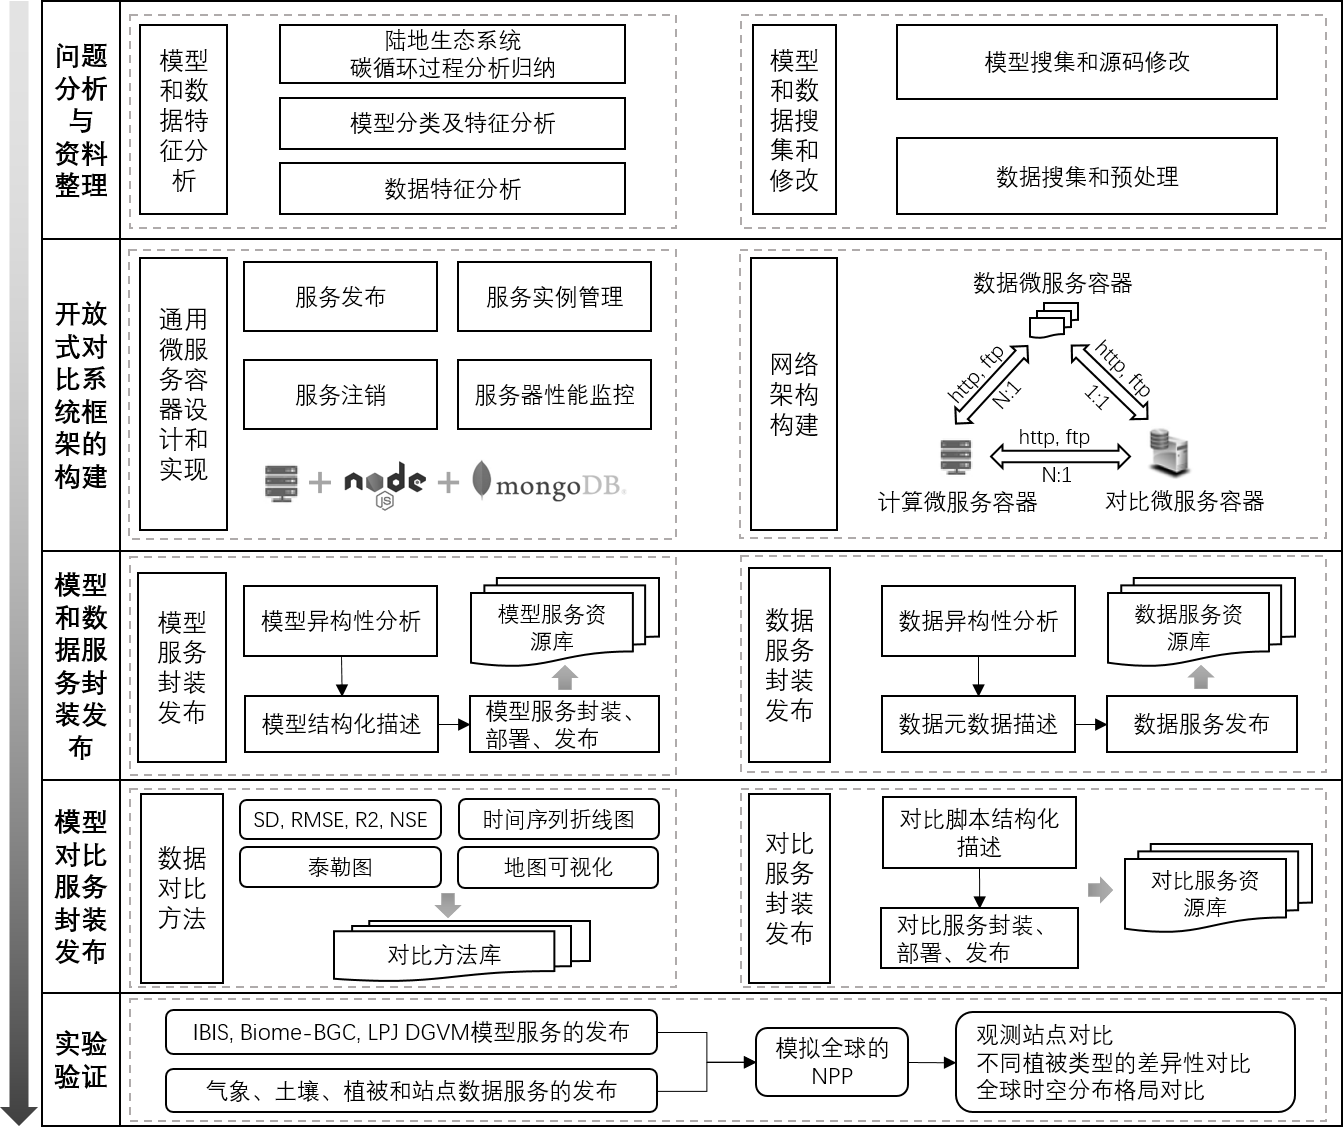
\includegraphics[width=1\textwidth]{tec-route}
    \caption{技术路线}
    \label{fig:tec-route}
\end{figure}

\section{论文组织结构}
第一章:绪论。介绍本文的研究背景和意义,梳理当前国内外的研究现状,得出模型对比是碳循环领域内的一个热点和难点,并提出了通过地理模型服务和数据服务集成的方法开展模型的对比,为模型对比提供了新的思路,在此基础上确定了本文的研究目标、研究内容、研究方法,并设计了具体的技术路线。

第二章:陆地生态系统碳循环模型对比分析。本章概述了陆地生态系统碳循环模型的概念、分类体系、结构和各类优缺点,介绍了碳循环模型运行相关的数据资源,具体分析了现有的模型对比方案的实现方式,并总结了其不足之处。

第三章:开放式陆地生态系统碳循环模型对比框架设计。本章从四个角度详细叙述了开放式的对比框架。首先从网络架构上设计了基于微服务的分布式网络,保证系统的解耦和稳定;其次,设计了微服务容器以支持模型微服务、数据微服务和对比微服务的发布,并详细介绍了模型资源组件、数据资源组件和对比资源组件的开放接口;再次,面向网络环境下对比过程的可共享和重用设计了模型对比方案描述语言;最后,从科学工作流执行流程的视角上,分析总结了对比的流程,并设计自动化执行引擎以驱动模型对比工作。

第四章:开放式对比资源接入方法。本章指出在开放式对比框架下,对比资源的开放式接入方法是系统的关键,并将对比资源分为数据资源、模型资源和对比方法资源三类。因此,本章分三个小节详细介绍三种资源的开放式接入方法。
对于数据资源,首先从格式、尺度和编排四个角度分析本文所用数据异构性特征,对领域通用标准数据设计结构化描述文档,对非标准数据采用示例数据URL的形式进行描述。然后遵循OGC WMS、WFS、WCS标准,使用GeoServer发布数据服务,并提供数据下载服务和数据处理服务;
对于模型资源,首先针对其特点进行分析,总结模型在参数策略、运行流程上的相同点和在开发层面的异构点。针对这些特征分三个视角进行结构化描述:面向人类理解的基本信息描述;面向机器调用的运行信息描述;面向模型部署的软硬件依赖环境描述。最后设计支持有源代码、无源代码和简单模型、集成模型的封装策略,在此基础上进行模型服务部署和发布。
对于对比资源,首先归纳总结在模型对比方面普遍使用的对比方法,包括有统计对比方法和可视化对比方法。然后将对比脚本看做与地理模型一样的可执行程序,采用同样的结构化描述和封装方法进行服务的封装和发布。

第五章:原型系统和案例验证。设计了开放式陆地生态系统碳循环模型对比系统,阐述了系统的网络架构、微服务容器和门户网站。基于此原型系统,从观测站点、植被功能类型和时空分布格局三点对IBIS、Biome-BGC和LPJ进行对比。

第六章:结论和展望。总结本文的研究结果,给出主要的研究结论和创新点,分析了论文研究中的不足之处,探讨未来的改进方向。